\documentclass[UTF8,11pt]{ctexart}
\usepackage[a4paper,margin=16mm]{geometry}
\usepackage{amsmath,amssymb}
\usepackage{booktabs,array}
\usepackage{graphicx}
\usepackage{xcolor}
\usepackage{enumitem}
\usepackage[hidelinks]{hyperref}

\setlength{\parindent}{0pt}
\setlength{\parskip}{0.55em}
\renewcommand{\arraystretch}{1.35}

\begin{document}

\begin{center}
{\Large \bfseries 2019 信号期末：移相法实现单边带调制题解}
\end{center}

\textbf{约定：}题图中 Hilbert 变换器输出记为
\[
x_h(t)=\mathcal{H}\{x(t)\},
\qquad
X_h(\omega)=H(j\omega)X(\omega).
\]
题目说明综合器下支路的极性可以自行选取。下面先按\textbf{下支路取加号}分析，即
\[
y(t)=y_2(t)+y_1(t).
\]
最后给出取减号时的结果。

\section*{1. Hilbert 变换器输出}

由题给
\[
H(j\omega)=
\begin{cases}
-j, & \omega>0,\\
j, & \omega<0.
\end{cases}
\]
因此
\[
X_h(\omega)=H(j\omega)X(\omega)
=
\begin{cases}
-jX(\omega), & \omega>0,\\
jX(\omega), & \omega<0.
\end{cases}
\]
也就是说，Hilbert 变换器\textbf{不改变幅度谱}，只把正频率移相 $-\pi/2$，负频率移相 $+\pi/2$。

\section*{2. 上支路频谱}

上支路
\[
y_2(t)=x(t)\cos \omega_c t.
\]
利用调制定理：
\[
Y_2(\omega)
=\frac{1}{2}\left[X(\omega-\omega_c)+X(\omega+\omega_c)\right].
\]
所以它是一个双边带抑制载波调制结果：在 $\omega=\omega_c$ 和 $\omega=-\omega_c$ 附近各有一份 $\frac12 X(\omega)$ 的搬移频谱。

\section*{3. 下支路频谱}

下支路
\[
y_1(t)=x_h(t)\sin \omega_c t.
\]
因为
\[
\sin\omega_c t=\frac{e^{j\omega_c t}-e^{-j\omega_c t}}{2j},
\]
所以
\[
Y_1(\omega)
=\frac{1}{2j}
\left[
X_h(\omega-\omega_c)-X_h(\omega+\omega_c)
\right].
\]

假设 $X(\omega)$ 的最高频率为 $\omega_m$，且 $\omega_c>\omega_m$。只看正频率载波附近：

\[
\begin{array}{c|c|c|c}
\text{频段} & Y_2(\omega) & Y_1(\omega) & Y_2(\omega)+Y_1(\omega)\\
\hline
\omega_c-\omega_m<\omega<\omega_c
& \frac12X(\omega-\omega_c)
& \frac12X(\omega-\omega_c)
& X(\omega-\omega_c)\\
\omega_c<\omega<\omega_c+\omega_m
& \frac12X(\omega-\omega_c)
& -\frac12X(\omega-\omega_c)
& 0
\end{array}
\]

因此当综合器取加号时，正频率处保留的是
\[
\omega_c-\omega_m<\omega<\omega_c,
\]
也就是\textbf{下边带 LSB}。负频率部分由实信号的共轭对称性对应出现。

\section*{4. 最终结论}

\textbf{若综合器下支路取加号：}
\[
y(t)=x(t)\cos\omega_c t+x_h(t)\sin\omega_c t,
\]
输出为\textbf{下边带调制信号 LSB}。

\textbf{若综合器下支路取减号：}
\[
y(t)=x(t)\cos\omega_c t-x_h(t)\sin\omega_c t,
\]
抵消关系相反，输出为\textbf{上边带调制信号 USB}。

\textbf{一句话记忆：}
在本题给定的 Hilbert 变换符号约定下，
\[
\boxed{x(t)\cos\omega_c t+x_h(t)\sin\omega_c t \Rightarrow \text{下边带}}
\]
\[
\boxed{x(t)\cos\omega_c t-x_h(t)\sin\omega_c t \Rightarrow \text{上边带}}
\]

\clearpage
\section*{5. 频谱图}

下图中用三角形基带谱作示意。形状只用于看清楚相加、相消关系；具体 $X(\omega)$ 只要是带限基带信号，结论相同。

\begin{center}
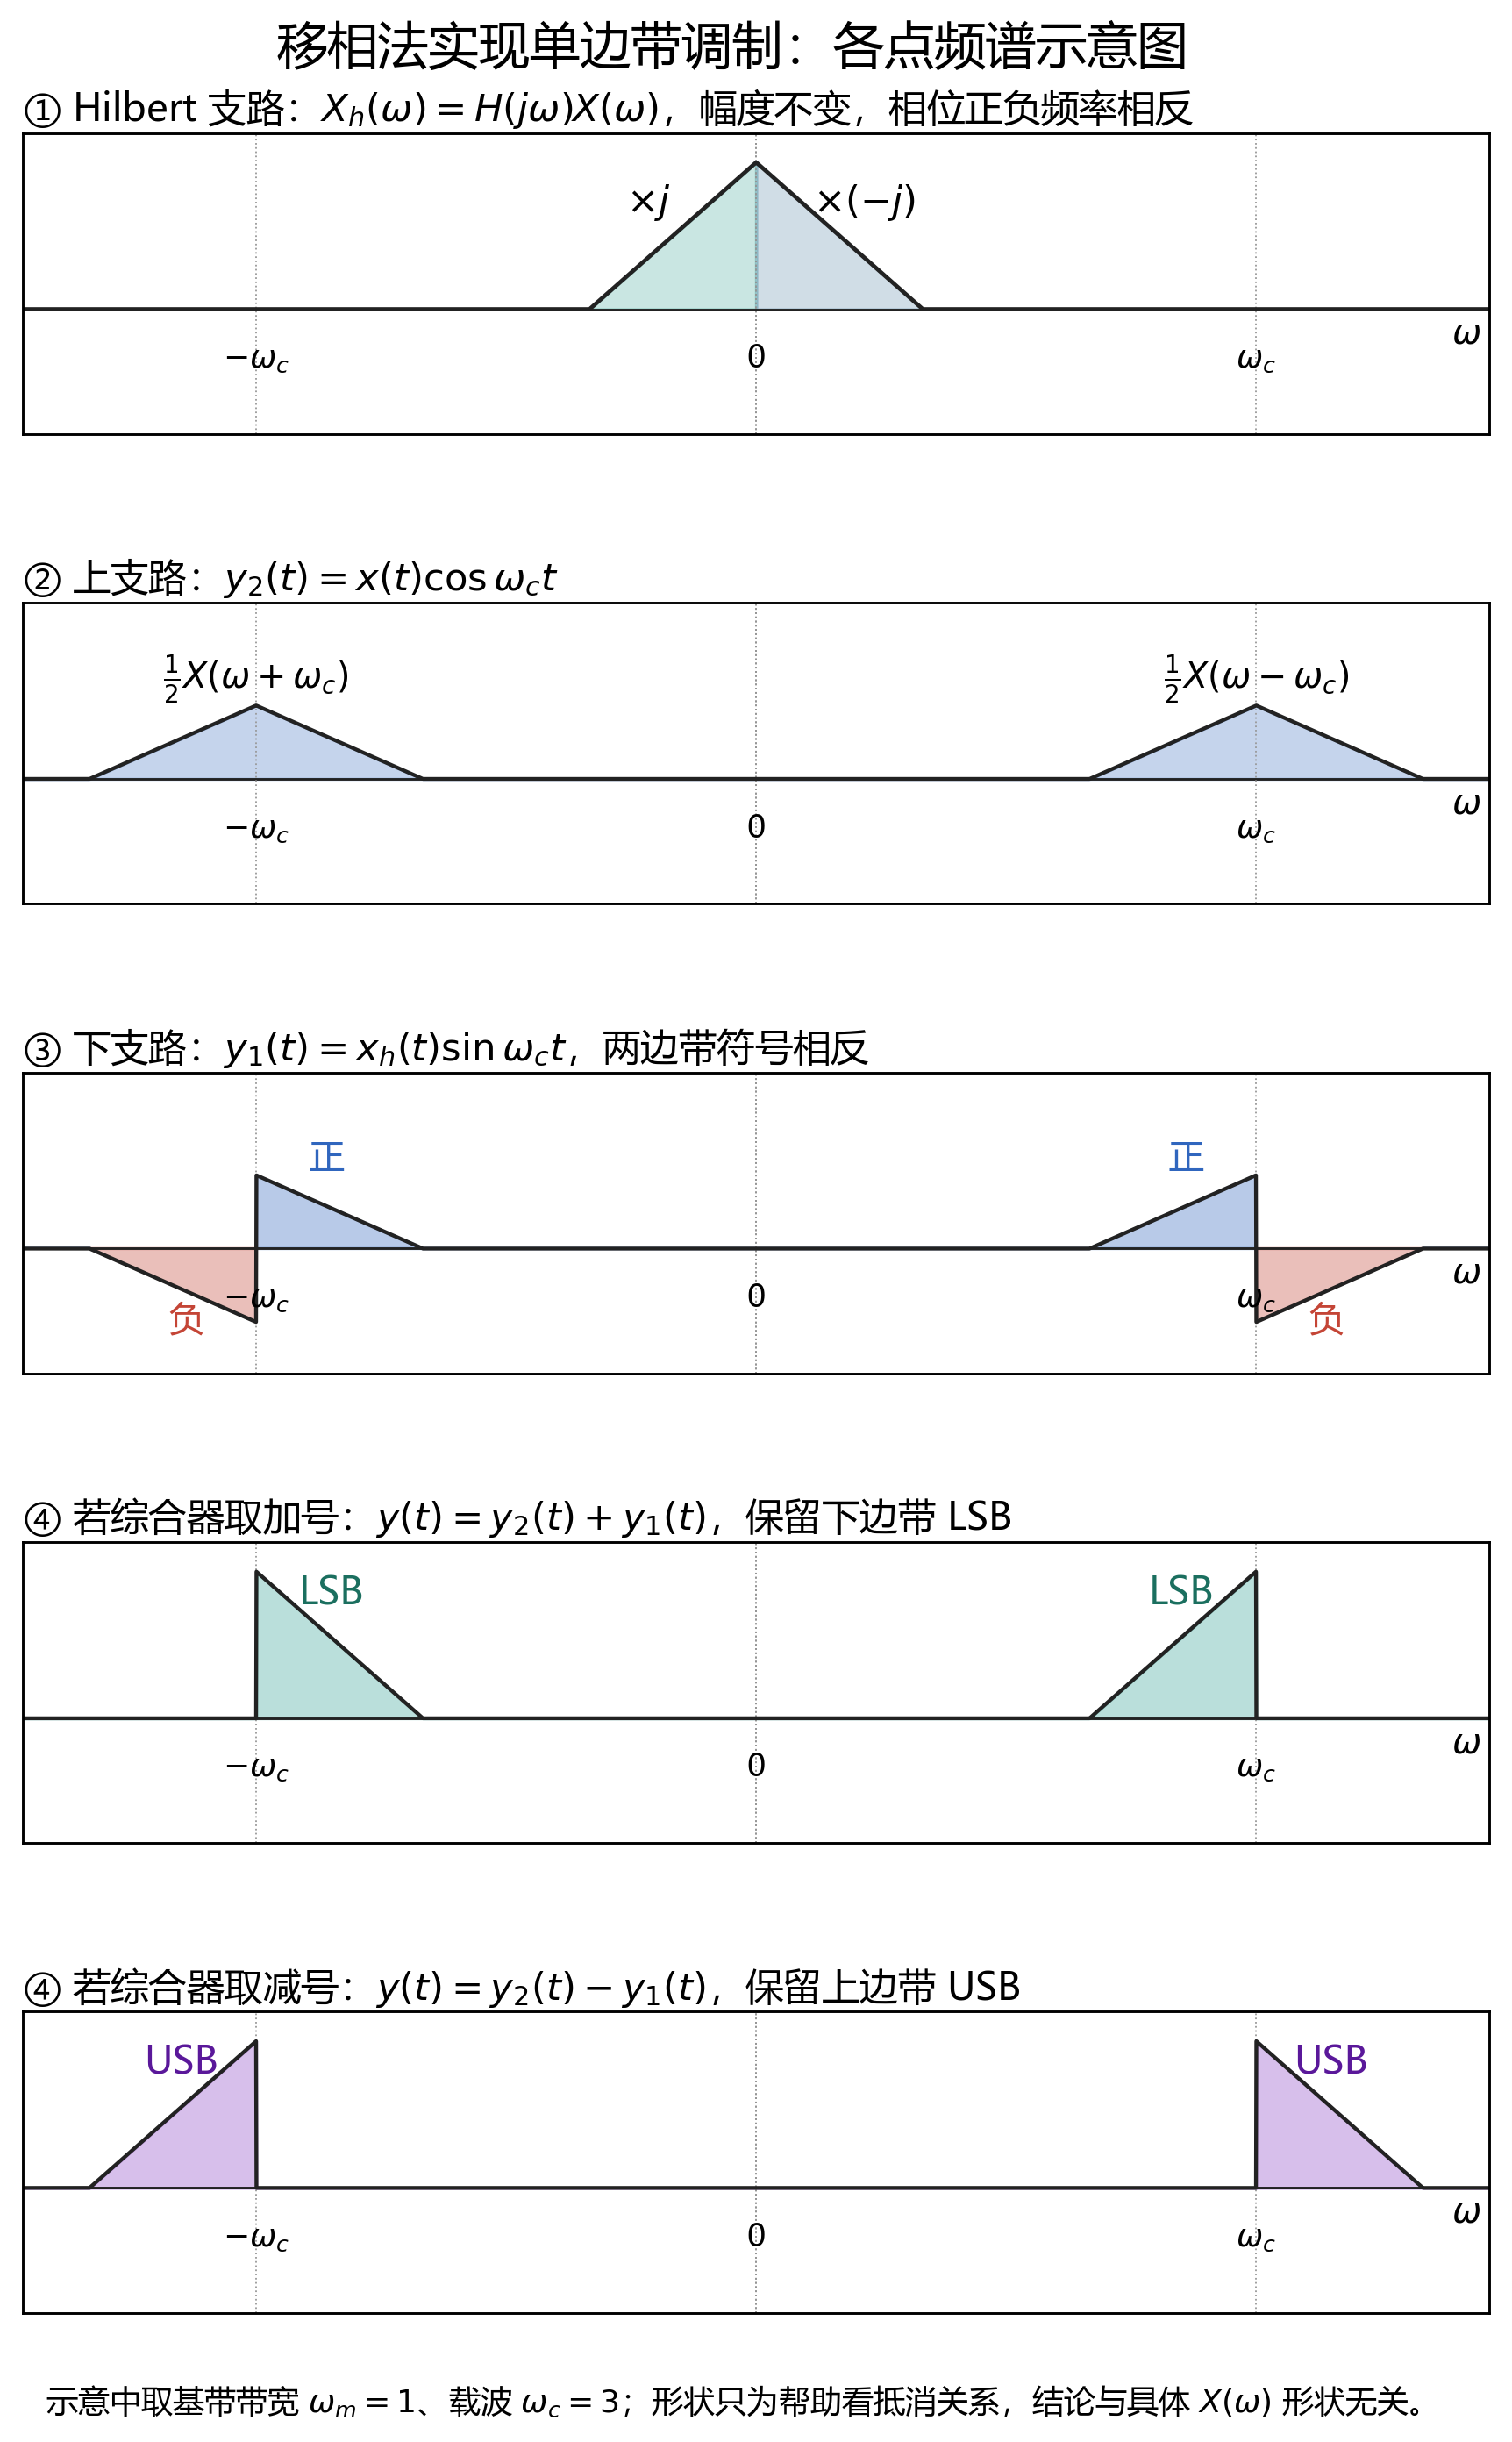
\includegraphics[height=0.88\textheight]{ssb_modulation_spectrum.png}
\end{center}

\end{document}
